This appendix provides the full test-set classification report and confusion matrix for each experimental run.
\subsection{LSTM}

\begin{figure}[H]
\centering

\includegraphics[width=0.62\textwidth]{../../src/lstm_evaluation_updated_full/confusion-matrix-regular-lstm.png}
\caption{Confusion matrix for LSTM.}
\end{figure}

\lstinputlisting[
    basicstyle=\ttfamily\scriptsize,
    numbers=none,
    frame=single,
    breaklines=true
]{../../src/lstm_evaluation_updated_full/classification_report-regular-lstm.txt}

\clearpage

\subsection{DistilBERT}
\begin{figure}[H]
\centering
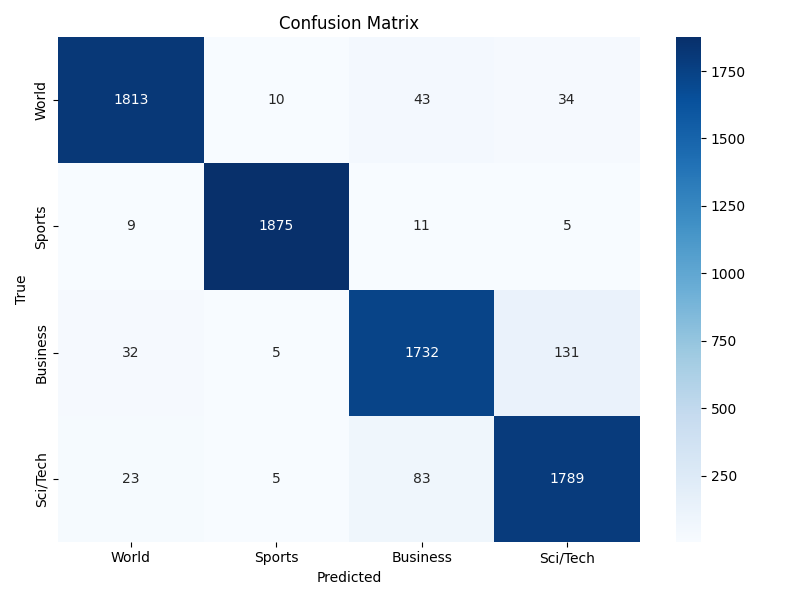
\includegraphics[width=0.62\textwidth]{../../src/bert_evaluation_full/confusion-matrix-regular-bert.png}
\caption{Confusion matrix for DistilBERT with maximum sequence length 128.}
\end{figure}

\lstinputlisting[
    basicstyle=\ttfamily\scriptsize,
    numbers=none,
    frame=single,
    breaklines=true
]{../../src/bert_evaluation_full/classification_report-regular-bert.txt}

\clearpage
% \subsection{CNN (Max Sequence Length: 256)}

% \begin{figure}[H]
% \centering
% 
\includegraphics[width=0.62\textwidth]{../../src/experiment_cnn_seq256/confusion_matrix_cnn.png}
% \caption{Confusion matrix for CNN with maximum sequence length 256.}
% \end{figure}

% \lstinputlisting[
%     basicstyle=\ttfamily\scriptsize,
%     numbers=none,
%     frame=single,
%     breaklines=true
% ]{../../src/experiment_cnn_seq256/classification_report.txt}

% \clearpage
% \subsection{LSTM (Max Sequence Length: 64)}

% \begin{figure}[H]
% \centering
% 
\includegraphics[width=0.62\textwidth]{../../src/experiment_lstm_seq64/confusion_matrix_lstm.png}
% \caption{Confusion matrix for LSTM with maximum sequence length 64.}
% \end{figure}

% \lstinputlisting[
%     basicstyle=\ttfamily\scriptsize,
%     numbers=none,
%     frame=single,
%     breaklines=true
% ]{../../src/experiment_lstm_seq64/classification_report.txt}

% \clearpage
% \subsection{LSTM (Max Sequence Length: 128)}

% \begin{figure}[H]
% \centering
% 
\includegraphics[width=0.62\textwidth]{../../src/experiment_lstm_seq128/confusion_matrix_lstm.png}
% \caption{Confusion matrix for LSTM with maximum sequence length 128.}
% \end{figure}

% \lstinputlisting[
%     basicstyle=\ttfamily\scriptsize,
%     numbers=none,
%     frame=single,
%     breaklines=true
% ]{../../src/experiment_lstm_seq128/classification_report.txt}

% \clearpage
% \subsection{LSTM (Max Sequence Length: 256)}

% \begin{figure}[H]
% \centering
% 
\includegraphics[width=0.62\textwidth]{../../src/experiment_lstm_seq256/confusion_matrix_lstm.png}
% \caption{Confusion matrix for LSTM with maximum sequence length 256.}
% \end{figure}

% \lstinputlisting[
%     basicstyle=\ttfamily\scriptsize,
%     numbers=none,
%     frame=single,
%     breaklines=true
% ]{../../src/experiment_lstm_seq256/classification_report.txt}
